% \begin{document}
\chapter{Livello di rete}
\section{Overview del libeello di rete}
\dfn{Livello di rete}{
    Il \textbf{livello di rete} (Network Layer) è responsabile del trasporto dei pacchetti da un host mittente a un host destinatario attraverso una o più reti intermedie, collandosi sopra il Data Link Layer e sotto il livello di trasporto
}

GLi obbiettivi princiapali del Network Layer sono:
\begin{itemize}
    \item \textbf{Modello di servizio}: definisce come il livello di rete fornisce il servizio ai livelli superiori
    \item \textbf{Instradamento e forwarding}:
    \begin{itemize}
        \item \textbf{Forwarding}: trasmissione di un pacchetto dall’ingresso di un router alla sua uscita appropriata.
        \item \textbf{Routing}: determinazione del percorso che i pacchetti devono seguire attraverso la rete.
    \end{itemize}
\end{itemize}

\subsection{Fuznioni del network layer}
Il Network Layer può essere suddiviso in due funzioni principali:
\begin{itemize}
    \item \textbf{Data Plane}: gestione del traffico dei pacchetti in tempo reale (forwarding)
    \item \textbf{Control Plane} (piano di controllo): determinazione del percorso ottimale per i pacchetti (routing)
\end{itemize}

Adesso vediamo entrambi nel dettaglio:

\subsubsection{Data Plane}
Il Data Plane è la parte del Network Layer responsabile della gestione effettiva del traffico dei pacchetti in tempo reale. A differenza del Control Plane, che decide il percorso dei pacchetti, il Data Plane si occupa di spostarli da un router all’altro fino alla destinazione.

Esistono due principali approcci alla gestione del Control Plane:

\begin{itemize}
    \item \textbf{Per-Router Control Plane}: ogni ruoter ha il proprio algoritmo di routing e prende decisioni autonomamente e comunicano tra di loro per scambiarsi informazioni di instradamento
    \begin{center}
        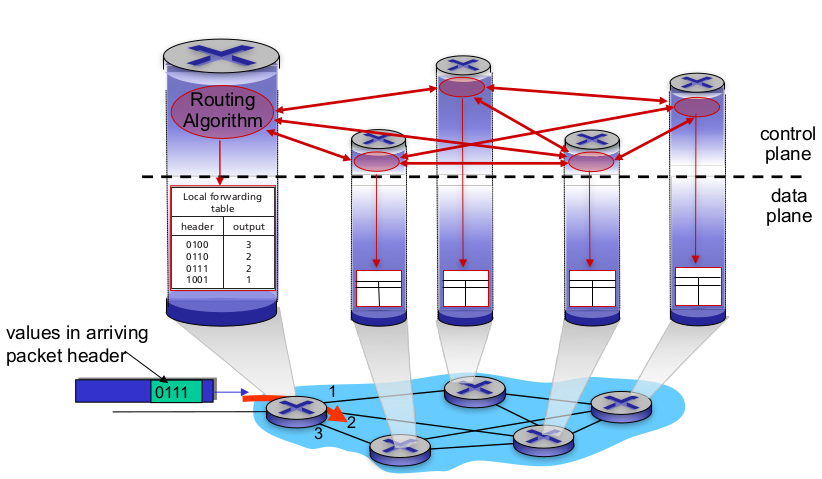
\includegraphics[width=10cm]{img/pre-router_control_plane.png}
    \end{center}
    \item \textbf{Logically Centralized Control Plane}: Un controller centralizzato (tipicamente remoto) prende le decisioni di instradamento e le comunica ai router, i router eseguono solo il forwarding senza prendere decisioni di routing
    \begin{center}
        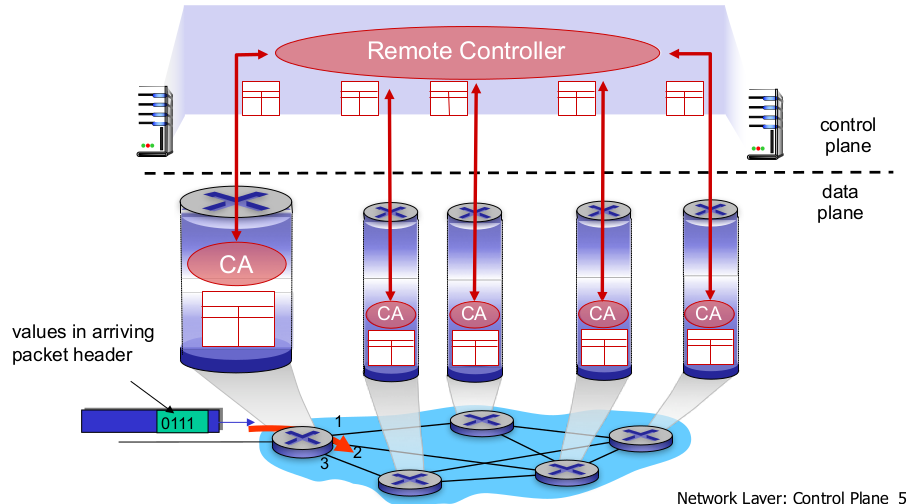
\includegraphics[width=10cm]{img/centralized_control_plane.png}
    \end{center}
\end{itemize}

In quasi tutte le infrastrutture di rete viene utilizzata il Logically Centralized Control Plane, mentre il Per-Router Control Plane viene utilizzata sopratutto nei sistemi di rete dinamici (ad esempio bluetooth col cellulare e altri dispositivi)

Fare le altre robe

\section{Router}

\section{IP datagram format}

\subsection{Frammentazione IP}

L'offset, le flag e l'identificatore permette la ricostruzione dell'intero pacchetto che era stato frammentato.

\ex{}{
  Supponiamo di avere:
  \begin{itemize}
  \item datagramma di 4000 byte
  \item MTU di 1500 byte
  \end{itemize}

  Ci servono 3 frammenti, che hanno lo stesso ID di pacchetto, il flag che indica i frammenti a 1 per i primi due e 0 per l'ultimo (proprio per indicare che e' l'ultimo) e gli offset (in byte/8 per compattezza).
}

\subsection{ATM}

Solo 5 byte, che sono un'etichetta di flusso, che serve per prenotare le risorse sul cammino determinato dal routing. I router che ricevono lungo il percorso leggono l'etichetta e sanno dove instradarli. E' l'emulazione di una commutazione di circuito fatto a pacchetto.

C'e' quindi un contratto a priori che garantisce una certa quantita' di flusso a disposizione.

La dimensione dei pacchetti ATM deve essere abbastanza piccolo da rendere veloce e gestibile la trasmissione, ma non troppo piccole da avere una porzione importante presa dall'header (overhead)

\section{IP addressing}
\ex{}{
  Reti di classe C
  Alto sx:
  \begin{itemize}
  \item rete di classe C
  \item Default Gateway 223.1.1.4, seguendo le best practices dovrebbe essere 223.1.1.254 (non 255 perche' sarebbe broadcast)
  \end{itemize}
  Per identificare la subnet in realta non si cambia la maschera perche boh
}

\ex{Subnets}{
  Ci sono 3 subnets, router separati per ogni sottorete connessi in modo completo (anello, ridontante). ma ci sono anche le reti degeneri che collegano i tre router, quindi in realta' ce ne sono 6 di reti.
}

\ex{DHCP}{
  Il DHCP server vede che arriva una richiesta in broadcast alla porta DHCP chiede al router se esiste un indirizzo e lo da al client. 

  Facendo spoofing del mac address, e' possibile apparire come una scheda di rete nuova ed e possibile spammare i DHCP in broadcast fino a esaurire gli IP.

  Tale attacco puo' essere fermato solo tramite autenticazione1
} 

\section{IPv6}
Non c'e' frammentazione, c'e' priorita' del flusso. Etichetta di flusso ci dice gia' la porta di destinazione, dato che per ogni flusso il router v6 salva la porta in una tabella separata.

\section{Forwarding Generalizzato}
Nelle SDN, abbiamo la possibilita' di definire su ogni router una politica locale nella quale abbiamo tre entita' di interesse:
\begin{itemize}
\item header
\item counter: controllo prestazioni
\item azioni: cosa fare se accade qualcosa
\end{itemize}

Le regole di gestione dei pacchetti sono semplici e generalizzati:
\begin{itemize}
\item azioni: 
\end{itemize}
% \end{document}
